\begin{frame}{TCP state machine}
\begin{itemize}
\item TIME\_WAIT, ESTABLISHED, \ldots?
\vspace{.5cm}
\item OS tracks ``state'' of TCP connection
    \begin{itemize}
    \item am I just starting the connection?
    \item is other end ready to get data?
    \item am I trying to close the connection?
    \item do I need to resend something?
    \end{itemize}
\item standardized set of state names
\end{itemize}
\end{frame}


\begin{frame}{TIME\_WAIT}
\begin{itemize}
\item remember delayed messages?
\vspace{.5cm}
\item problem for TCP ports
\item if I reuse port number, I can get message from old connection
\item solution: TIME\_WAIT to make sure connection really done
    \begin{itemize}
    \item done after sending last message in connection
    \end{itemize}
\end{itemize}
\end{frame}

\begin{frame}{TCP state machine picture}
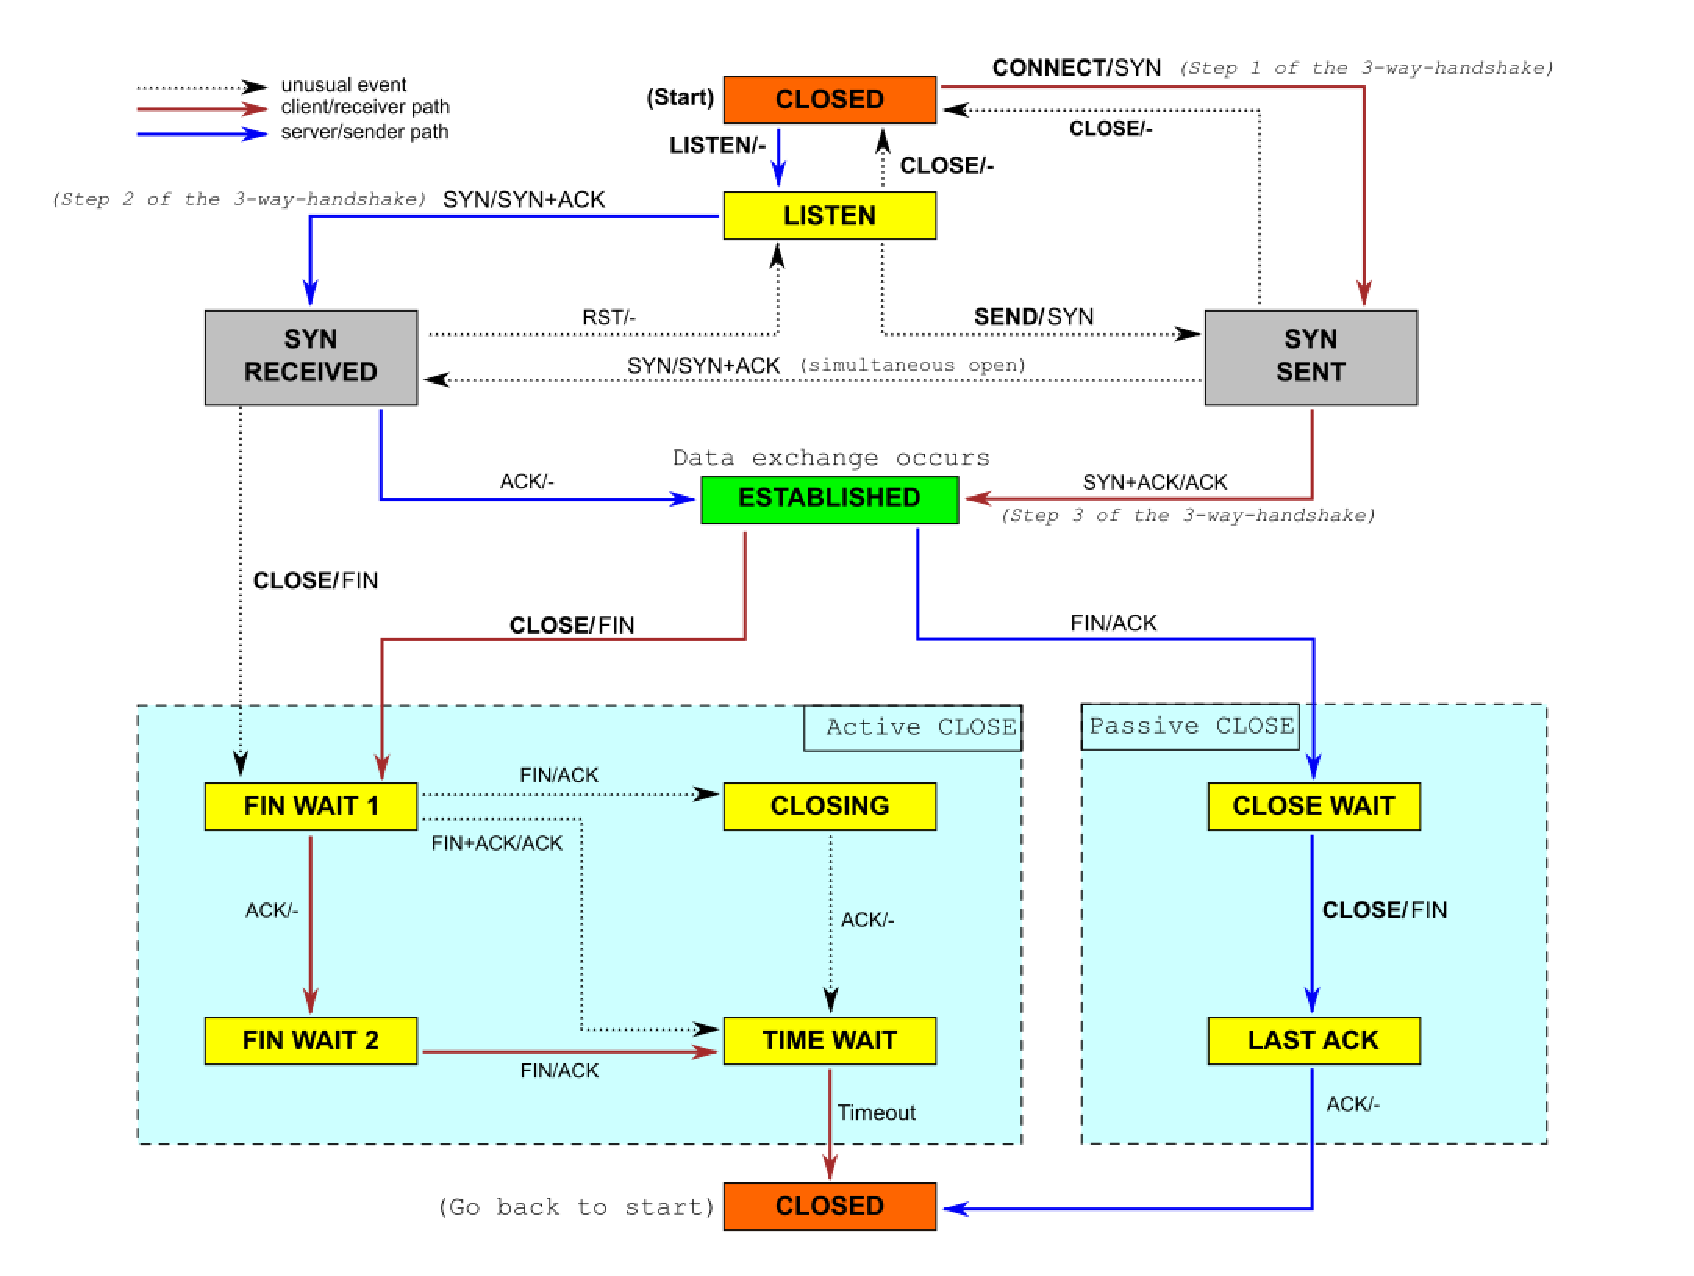
\includegraphics[height=0.9\textheight]{TcpState}
\imagecredit{via Wikimedia/User:Scil100; CC-BY-SA}
\end{frame}
